% Copyright 2004 by Till Tantau <tantau@users.sourceforge.net>.
%
% In principle, this file can be redistributed and/or modified under
% the terms of the GNU Public License, version 2.
%
% However, this file is supposed to be a template to be modified
% for your own needs. For this reason, if you use this file as a
% template and not specifically distribute it as part of a another
% package/program, I grant the extra permission to freely copy and
% modify this file as you see fit and even to delete this copyright
% notice. 

\documentclass{beamer}

% There are many different themes available for Beamer. A comprehensive
% list with examples is given here:
% http://deic.uab.es/~iblanes/beamer_gallery/index_by_theme.html
% You can uncomment the themes below if you would like to use a different
% one:
%\usetheme{AnnArbor}
%\usetheme{Antibes}
%\usetheme{Bergen}
%\usetheme{Berkeley}
%\usetheme{Berlin}
%\usetheme{Boadilla}
%\usetheme{boxes}
%\usetheme{CambridgeUS}
%\usetheme{Copenhagen}
%\usetheme{Darmstadt}
%\usetheme{default}
%\usetheme{Frankfurt}
%\usetheme{Goettingen}
%\usetheme{Hannover}
%\usetheme{Ilmenau}
%\usetheme{JuanLesPins}
%\usetheme{Luebeck}
%\usetheme{Madrid}
%\usetheme{Malmoe}
%\usetheme{Marburg}
%\usetheme{Montpellier}
%\usetheme{PaloAlto}
%\usetheme{Pittsburgh}
%\usetheme{Rochester}
%\usetheme{Singapore}
%\usetheme{Szeged}
\usetheme{Warsaw}

\usepackage[brazil]{babel}
\usepackage[utf8]{inputenc}
\usepackage{graphicx,caption}

% Add page to template
\addtobeamertemplate{navigation symbols}{}{%
    \usebeamerfont{footline}%
    \usebeamercolor[fg]{footline}%
    \hspace{1em}%
    \insertframenumber/\inserttotalframenumber
}

\title[Colab - Um framework de Integração de Aplicações Web]
{Colab - Um framework de Integração de\\Aplicações Web: Desenvolvimento e Aplicação}

% A subtitle is optional and this may be deleted
\subtitle{Exame de Qualificação}

\author[Sérgio Oliveira Campos (ICMC) – 2016]{Sérgio Oliveira Campos\inst{1}\\{\small Orientador: Prof. José Carlos Maldonado\inst{1}}\\{\small Orientador: Prof. Paulo Meirelles\inst{2}}}
% - Give the names in the same order as the appear in the paper.
% - Use the \inst{?} command only if the authors have different
%   affiliation.

\institute[ICMC] % (optional)
{
  \inst{1}%
  Instituto de Ciências Matemáticas e de Computação – ICMC\\
  Universidade de São Paulo
  \and
  \inst{2}%
  Faculdade de Engenharias do Gama – FGA\\
  Universidade de Brasília
}
% - Use the \inst command only if there are several affiliations.
% - Keep it simple, no one is interested in your street address.

\date{Maio 2016}
% - Either use conference name or its abbreviation.
% - Not really informative to the audience, more for people (including
%   yourself) who are reading the slides online

\logo{
\includegraphics[height=0.7cm]{logo_icmc.png}}

%\subject{Theoretical Computer Science}
% This is only inserted into the PDF information catalog. Can be left
% out. 

% If you have a file called "university-logo-filename.xxx", where xxx
% is a graphic format that can be processed by latex or pdflatex,
% resp., then you can add a logo as follows:

\pgfdeclareimage[height=0.5cm]{university-logo}{logo_icmc.png}
\logo{\pgfuseimage{university-logo}}

% Delete this, if you do not want the table of contents to pop up at
% the beginning of each subsection:
%\AtBeginSubsection[]
%{
%  \begin{frame}<beamer>{Outline}
%    \tableofcontents[currentsection,currentsubsection]
%  \end{frame}
%}

% Let's get started
\begin{document}

\begin{frame}{Sumário}
  \tableofcontents
  % You might wish to add the option [pausesections]
\end{frame}

% Section and subsections will appear in the presentation overview
% and table of contents.
\section{Introdução}

\subsection{Contexto}

\begin{frame}{Contextualização}

  \begin{itemize}
  \item {
    A Web como plataforma \cite{OReilly2007}
  }
  \item{
    Computação em nuvem
  }
  \item {
    Crescente uso de aplicações Web
  }
  \end{itemize}
 
\end{frame}


\begin{frame}{Problema}

  Dificuldade para os usuários:  
  \begin{itemize}
  \item {
    Aprender a utilizar múltiplas ferramentas
  }
  \item {
    Recordar múltiplas credenciais de acesso
  }
  \item {
    Ações redundantes entre ferramentas
  }
  \end{itemize}
\end{frame}

\begin{frame}{Problema}
  Dificuldades para as organizações:
  \begin{itemize}

  \item {
    Trabalhar com conjuntos de dados redundantes
  }
  \item {
    Garantir a segurança de múltiplos sistemas
  }
  \item {
    Visualizar e cruzar informações vindas de sistemas distintos
  }
  \item {
    Evitar inconsistência
  }
  
  \end{itemize}
\end{frame}

\subsection{Objetivo}

\begin{frame}{Objetivo}
    \begin{block}{Proposta}
        Desenvolver um framework para apoiar o processo de integração de famílias de web sites com o objetivo de unificar a experiência do usuário e reduzir as inconsistências de dados.
    \end{block}
    
    Metas:
    \begin{itemize}
        \item{Integrar aplicações existentes}
        \item{Simplificar o processo de integração}
        \item{Permitir que as aplicações sejam atualizadas com menor impacto possível}
    \end{itemize}
\end{frame}

\subsection{Trabalhos Relacionados}

\begin{frame}{Trabalhos Relacionados}
  \begin{itemize}
  \item {Mashup \cite{Yu2007} \cite{Yu2008} \cite{Daniel2011}}
  \item {Famílias de Web site\cite{Eichinger2009}}
  \item {Proxies de autenticação \cite{Takada2012}}
  \end{itemize}
\end{frame}

\subsection{Terminologia e Conceitos}

\begin{frame}[allowframebreaks]{Terminologia e Conceitos}
  \begin{itemize}
    \item{
        \textbf{HTTP:} protocolo de camada de aplicação utilizado como base para a construção da web e é o principal protocolo implementado pelos navegadores. Utiliza o modelo cliente-servidor onde cada requisição e resposta são compostos por corpo (\textit{body}) e cabeçalhos (\textit{headers}). É um protocolo sem estado (\textit{stateless}).
    }
    \framebreak
    \item{
       \textbf{Famílias de web sites:} \textit{``Web Site Families organize related web sites in a hierarchy in which common design requirements for members at a lower level (e.g., department web site) are defined at the higher level (e.g., faculty level).''} \cite{Eichinger2009}
    }
    
    \item{
        \textbf{Single Sing-On:} uma propriedade de sistema de controle de acesso que permite que um usuário se autentique em múltiplos sistemas fornecendo suas credenciais apenas uma vez. O SSO é uma solução que fornece boa usabilidade e segurança \cite{Pashalidis2003}.
    }
    
    \framebreak
    \item{
        \textbf{Evento:} uma ocorrência em uma aplicação que pode ser tratada pela própria aplicação ou por outras aplicações.
    }
    
    \item{
        \textbf{Middleware:} sistema responsável por intermediar a comunicação entre outros dois sistemas, adicionando funcionalidades até então inexistentes. Um exemplo de middleware são as aplicações Proxy.
    }
    
    \framebreak
    \item{
        \textbf{Proxy:} sistema responsável por intermediar a comunicação entre aplicações do tipo cliente-servidor com um ou mais objetivos explícitos como caching ou segurança na transmissão de informações.
    }
    
    \item{
        \textbf{Message-Oriented Middleware (MOM):} aplicações utilizadas para intermediar a comunicação de sistemas distribuídos através da troca de mensagens \cite{Vinoski2006}.
    }
    
    \framebreak
    \item{
        \textbf{Application Programming Interface (API):} interfaces de um programa que permitem que outro programa interaja com ele. As APIs podem ser locais (como no caso de bibliotecas do sistema operacional ou drivers), ou remotas (e.g.: web services).
    }
    
    \item{
        \textbf{Common Gateway Interface (CGI):} padrão que permite que aplicações instaladas em um determinado servidor gerem, de forma dinâmica, páginas HTML para que um servidor HTTP possa servi-las \cite{robinson2004rfc}.
    }
    
    \framebreak
    \item{
        \textbf{Template (aplicação web):} são mecanismos que permitem que conteúdo dinâmico seja inserido em páginas HTML, a princípio estáticas.
    }
    
    \item{
        \textbf{Plugin:} artefato de software que adiciona funcionalidade à uma aplicação. Os plugins normalmente são implementados utilizando uma API específica da própria aplicação. A utilização de plugins permite que programadores não envolvidos na criação de uma aplicação possam adicionar funcionalidades e realizar customizações sem a alteração do código principal dela.
    }
  \end{itemize}
\end{frame}

\section{Integrações}

\begin{frame}{Colab}
  O framework atua como:
  \begin{itemize}
      \item {
        Servidor de integrações
      }
      \item {
        Barramento de comunicação
      }
  \end{itemize}
  
  \hfill \break

  Com o objetivo de integrar:
  \begin{itemize}
      \item {
        Autenticação
      }
      \item {
        Visual
      }
      \item{
        Eventos
      }
      \item{
        Dados e busca
      }
  \end{itemize}
\end{frame}

\begin{frame}{Colab - Proxy Reverso}
  \begin{center}
    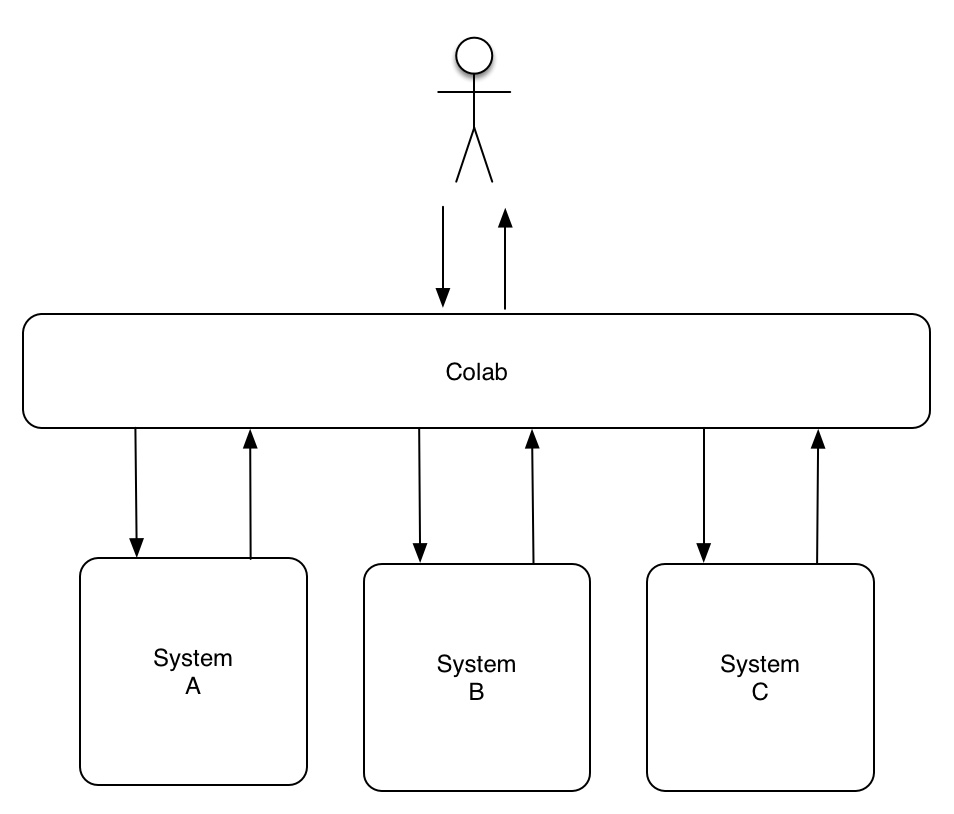
\includegraphics[height=6cm]{colab-basics}
  \end{center}
\end{frame}

\subsection{Autenticação}

\begin{frame}{Integração de Autenticação}

  \textbf{Autenticação}: método para verificar a identidade de um usuário.

  \hfill \break

  Diferentes formas de autenticação:

  \begin{itemize}
  \item {
    Usuário e senha
  }
  \item {
    Token
  }
  \item{
    Certificados digitais
  }
  \item{
    Whitelist
  }
  \end{itemize}
\end{frame}

\begin{frame}{Integração de Autenticação}
  Formas de integração:
  \begin{itemize}
    \item{Compartilhamento de credenciais de acesso}
    \item{Federação: OpenID, OAuth, Facebook Connect}
    \item{\textit{Single Sign-On} (SSO)}
    \item{Variável REMOTE\_USER (CGI)} \cite{robinson2004rfc}
  \end{itemize}
\end{frame}

\begin{frame}{Integração de Autenticação}
  Injeção de REMOTE\_USER
  \begin{center}
    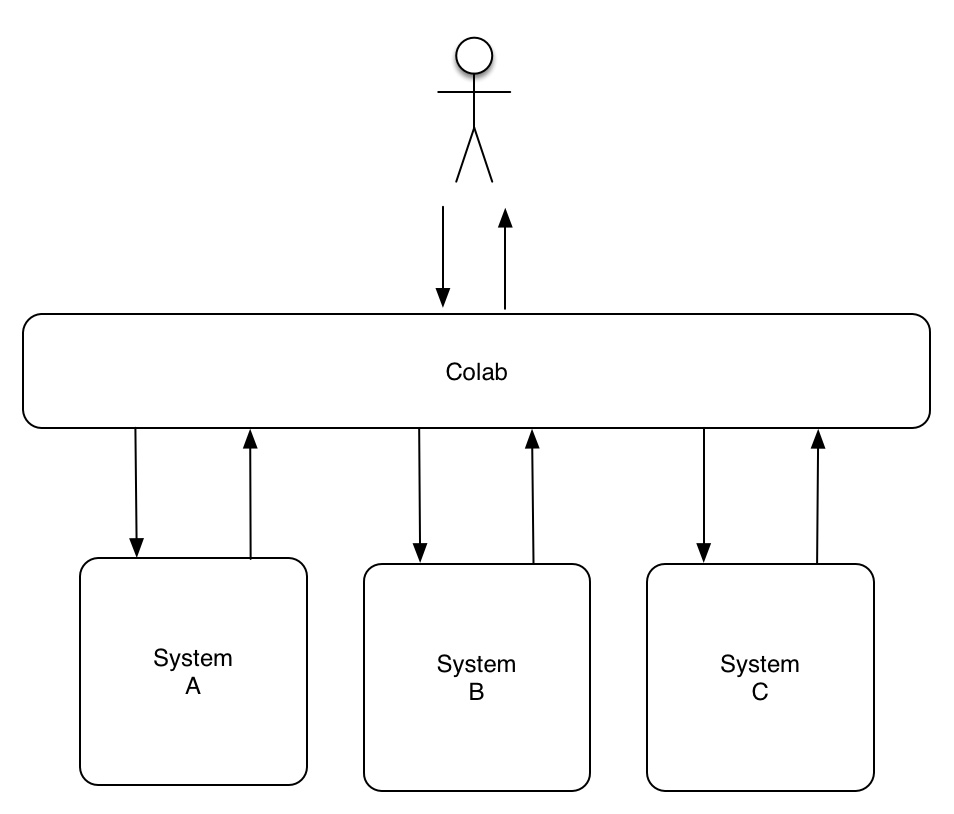
\includegraphics[height=5cm]{colab-basics}
  \end{center}
\end{frame}

\begin{frame}{Integração de Autenticação}
  Injeção de REMOTE\_USER
  \begin{enumerate}
    \item{Verificar se a sessão pertence a um usuário diferente:}
    \begin{itemize}
        \item{\textbf{Sim:} Encerra a sessão do usuário}
    \end{itemize}
    
    \item{Verificar se o usuário já existe:}
    \begin{itemize}
        \item{\textbf{Sim:} Realiza a autenticação}
        \item{\textbf{Não:} Cria o usuário e realiza a autenticação}
    \end{itemize}
  \end{enumerate}
  Caso o REMOTE\_USER venha vazio a sessão deve ser encerrada.
\end{frame}


\subsection{Visual}

\begin{frame}{Integração Visual}

  Tecnologias Básicas:
  \begin{itemize}
  \item {
    HTML
  }
  \item {
    CSS
  }
  \item {
    Javascript
  }
  \end{itemize}

  \hfill \break

  Tipos de template utilizados na Web:
  \begin{itemize}
  \item {
    Server-side \cite{Garcia-Izquierdo2012}
  }
  \item {
    Client-side \cite{Garcia-Izquierdo2012}
  }
  \item {
    Edge-side include (ESI) \cite{Brodie2004}
  }
  \end{itemize}
\end{frame}


\begin{frame}{Integração Visual}
  Injeção de conteúdo (Diazo)
  \hfill \break
  
  Artefatos do Diazo:
  \begin{itemize}
    \item{Template (HTML)}
    \item{Conteúdo (HTML)}
    \item{Regras (XSLT)}
    
    \item{Processador}
  \end{itemize}
\end{frame}

\begin{frame}{Integração Visual}
  Funcionamento Diazo
  \begin{center}
    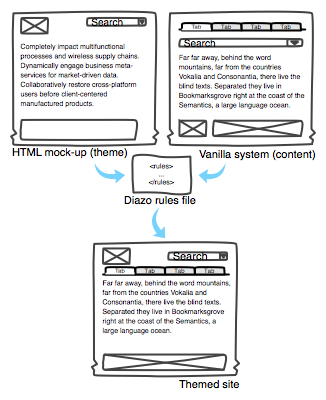
\includegraphics[height=5cm]{diazo-concept}
  \end{center}
  \scriptsize Fonte:\thinspace{http://docs.diazo.org/ (2014)}

\end{frame}

\subsection{Eventos}

\begin{frame}{Integração por Eventos}

  Implementação baseada me Message-Oriented Middleware (MOM).
  \hfill \break

  Exemplo de operação:
  \begin{itemize}
  \item {
    A aplicação X emite um evento
  }
  \item {
    O evento é registrado pelo MOM
  }
  \item{
    A aplicação Y está escutando pelo evento enviado e pode reagir a ele. 
  }
  \item{
    Outras aplicações que não ouviam pelo sinal não são afetadas diretamente.
  }
  \end{itemize}
\end{frame}

\begin{frame}{Integração por Eventos}

  A implementação dos eventos é feita através do uso de plugins:
  \begin{itemize}
  \item {
    Cada aplicação integrada possui seu próprio plugin.
  }
  \item{
    O plugin é o componente responsável por conhecer as aplicações integradas e decidir quais devem ser emitidos e quais sinais devem ser ouvidos.
  }
  \item{
    Um sinal pode resultar na emissão de novos sinais (permite a existência de um plugin com responsabilidade exclusiva de controlador).
  }
  \end{itemize}
\end{frame}

\subsection{Dados e Busca}

\begin{frame}{Integração de Dados e Busca}
  A integração de dados centraliza os dados das aplicações integradas em uma única base.
  \hfill \break

  \begin{itemize}
  \item {
    Facilita a consulta por aplicações externas.
  }
  \item {
    Possibilita um mecanismo de busca centralizado.
  }
  \item {
    Permite tratamento e mineração de dados.
  }
  \end{itemize}
\end{frame}

\begin{frame}{Integração de Dados e Busca}
  
  Funcionamento:

  \begin{itemize}
  \item {
    A leitura dos dados (indexação) é realizada através da chamada de métodos que são implementados em plugins.
  }
  
  \item{
    Modelo de dados e de busca também devem ser implementados no plugin.
  }
  
  \item {
    O carregamento dos dados ocorre de forma periódica.
  }
  \end{itemize}
\end{frame}

\subsection*{Estado atual}

\begin{frame}{Colab - Plugins}
  \begin{center}
    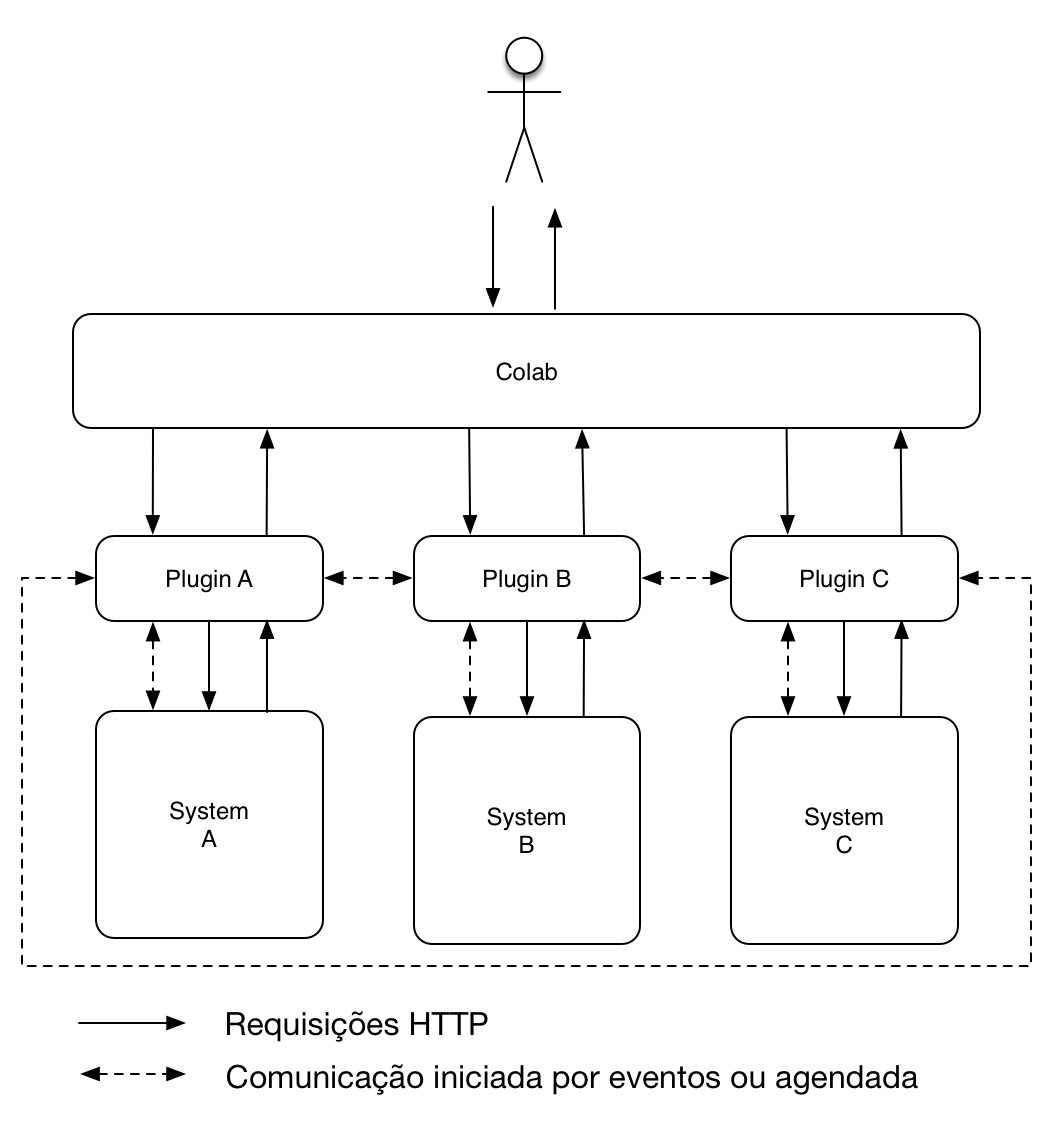
\includegraphics[height=6.0cm]{colab-plugins}
  \end{center}
\end{frame}

\section{Limitações}

\begin{frame}{Limitações do Trabalho}
  \begin{itemize}
  \item {
    Ponto único de falha.
  }
  \item {
    Dificuldade de operação em tempo real.
  }
  \item {
    Aumento da latência das requisições.
  }
  \item{
    Dificuldade de integração.
  }
  \item{
    Aplicações precisam suportar o uso de REMOTE\_USER.
  }
  \end{itemize}
\end{frame}

\section{Plano de trabalho}

\begin{frame}{Plano de Trabalho}
    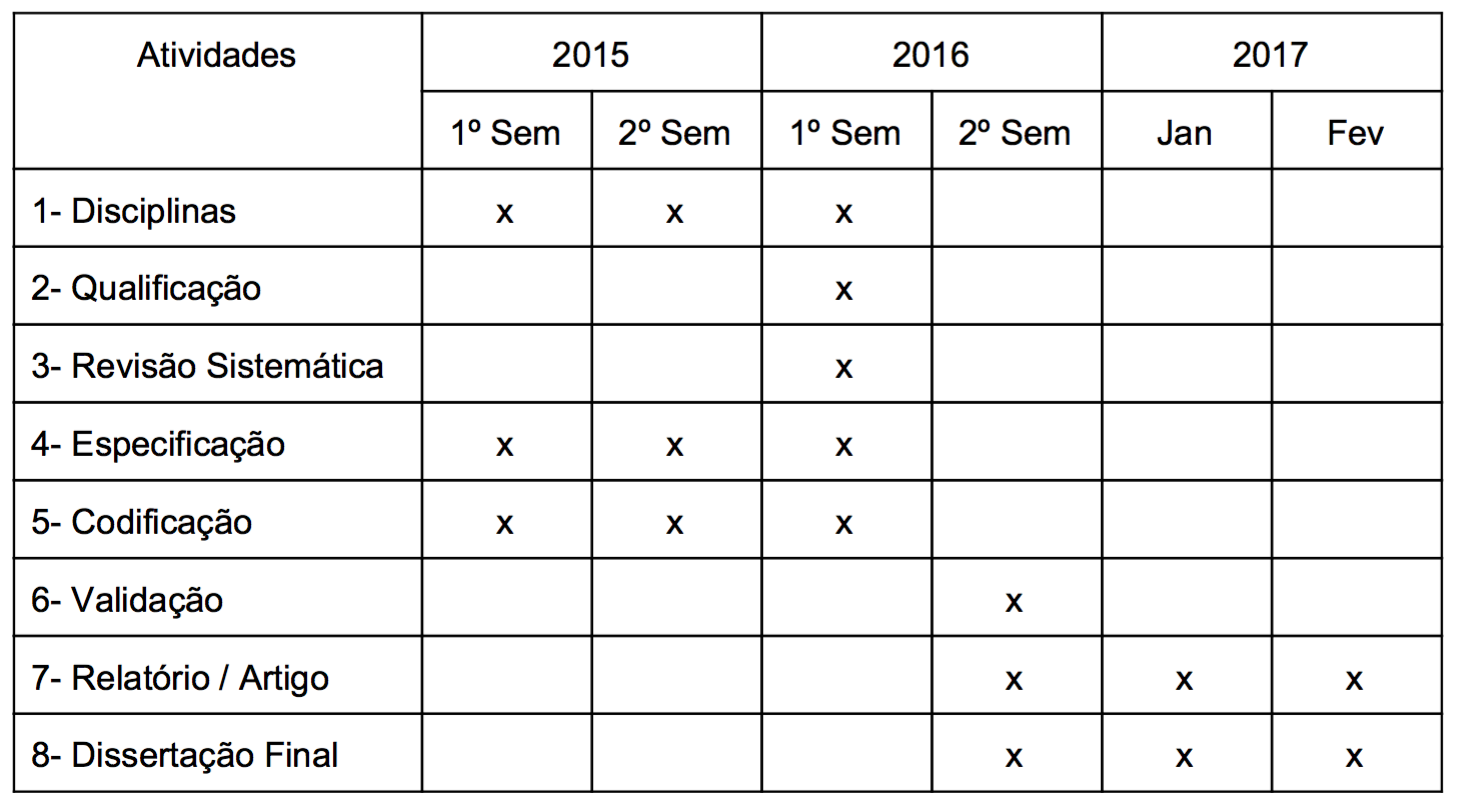
\includegraphics[scale=0.4]{plano_de_trabalho}
\end{frame}

% All of the following is optional and typically not needed. 
\section*{Referências}

\begin{frame}[allowframebreaks]
    \frametitle{Referências}
    \bibliographystyle{apalike}
    \bibliography{references.bib}
\end{frame}

\end{document}